% 1. EDIT COURSE SPECIFIC PARAMETERS (these)
\def \instructor{arciero}
\def \coursenum{150 B,C}
\def \coursename{Statistics for Life Sciences}




\def \callnumber{}  % and   20225
\def \year{2023}
\def \room{}
\def \daytime{}



\def \prerequisite{LAC 022 or SAS 022 or UL4 mathematics placement}
\def \website{Brightspace \url{https://brightspace.une.edu/d2l/home/59742}}

\newif\ifquiz
\quizfalse


\newif\ifpart
\partfalse


\newif\ifhw
\hwtrue



% 2. EDIT (IF CHANGES) GLOBAL INCLUDE FILES (e.g., academic integrity)
%\newcommand{\globalpath}{global_inc}  % path to global folder

\documentclass[12pt]{files/handoutX}


% --------------- RUN -------------- %




%\usepackage{add-copyright}
\usepackage{geometry}
\geometry{margin=0.8in,top=0.4in,bottom=0.75in}


\usepackage{mathabx, color} % square bullets in itemized list

\renewcommand{\labelitemi}{
\includegraphics[]{files/blue_bullet2.png}}


 

\usepackage[T1]{fontenc}
\usepackage{lmodern}
\usepackage{hyperref}
\usepackage{nopageno}
\usepackage{multicol}
\usepackage[final]{pdfpages}
%\geometry{margin=1cm}


\newcommand{\peem}{\textsc{p.m.}}
\newcommand{\ayem}{\textsc{a.m.}}

%\titlespacing*{\section}{0in}{*0}{*1}
%\titlespacing*{\subsection}{0in}{*0}{*1}


\usepackage{tabularx}
\usepackage{rotating}

\setlength{\parindent}{0in}
\setlength{\parskip}{0in}
\usepackage{calc}







%\title{\includegraphics[scale=0.6]{\globalpath/UNE_logo}}
\title{Statistics for Life Sciences}
% header information
\author{Fall \year}
\course{MAT\coursenum}
\date{\bf  }

%\usepackage[T1]{fontenc}
%\usepackage{lmodern}
%\usepackage{hyperref}
%\usepackage{nopageno}
%\usepackage{multicol}
%\geometry{margin=1cm}


%\newcommand{\peem}{\textsc{p.m.}}
%\newcommand{\ayem}{\textsc{a.m.}}

%\titlespacing*{\section}{0in}{*0}{*1}
%\titlespacing*{\subsection}{0in}{*0}{*1}


\usepackage{tabularx}
\usepackage{rotating}

\setlength{\parindent}{0in}
\setlength{\parskip}{0.0in}
\usepackage{calc}





\begin{document}
\maketitle



\subsection*{Course Information}
%\vspace{1ex}%
\noindent\parbox{0.5\textwidth}{%
	\noindent\begin{tabular}{@{}ll}
		\textsf{Course:} & MAT \coursenum \,$-$ \coursename \\
%\textsf{Call \#:} & \callnumber \\
%\textsf{Room:} & \room \\

\textsf{Meets:} & Section B: Monday, Thursday 12:30 - 1:50 Decary 336 \\
 & Section C: Monday, Thursday 2:00 - 3:20 Decary 336 \\


\textsf{Prerequisites:} & \prerequisite \\


\textsf{Text:} & {\it OpenIntro Statistics}, 4ed, D. Diez, M. Cetinkaya-Rundel, C. Barr,\\

&  Creative Commons, freely available: \url{https://leanpub.com/os} \\
& (select ``The Book" only, set price to zero (or contribute) and download pdf) \\

\textsf{Supplementary text:} & {\it Introduction to Modern Statistics}, M. Cetinkaya-Rundel, J. Hardin,  \\
& Creative Commons, free web based: https://openintro-ims.netlify.app/index.html \\



\textsf{Course Website:} & \website \\
%\textsf{Computation Site:} & \url{https://cloud.sagemath.com} \\
% \textsf{Homework Website:} & \homework   \\





\end{tabular}}


\subsection*{Instructor Information}
%\vspace{1ex}%
\noindent\parbox{0.5\textwidth}{%
	\noindent\begin{tabular}{@{}ll}
		\input{files/\instructor}
\end{tabular}}

\subsection*{Course description}
In this course, students apply principles of research design and statistics to analyze and interpret data and draw conclusions about experimental situations relevant to the sciences. Topics include random sampling, graphic and numeric descriptive data analysis, the normal distribution, hypoth- esis testing, t-tests, analysis of variance, correlation, and regression. Students will use statistical software to examine data graphically and perform statistical analyses.








\subsection*{Learning outcomes}

At the conclusion of this course students will be able to:

\begin{itemize}
	\item Distinguish among different types of data.
	\item Describe a variety of random sampling methods.	
	\item Summarize data verbally, numerically, symbolically, and/or graphically to effectively communicate the results of data analysis. 
	\item Perform inferential hypothesis testing, including t-tests, analysis of variance, correlation, and regression.
	\item Recognize some sources of bias and limitations of statistical analysis and inferences.


%	\item Apply the understanding of statistics to interpret and evaluate research reported by others.


%item Discuss and present statistical analysis, including methods, results, conclusions, and justifi- cations based on supporting evidence in both verbal and written formats.

\end{itemize}


\subsection*{Course in the Curriculum}


This course is part of the Core Curriculum that is taken by UNE undergraduates and provides a foundation in key themes in the liberal arts. It addresses the Mathematics component of the Core Curriculum and the following learning outcomes:
\begin{itemize}
	\item Apply mathematical reasoning to formulate and solve problems in mathematics and other disciplines,
\item Interpret mathematical information and draw informed conclusions, and
\item Communicate mathematically using symbolic, numerical, and graphical representa-
	tions.
\end{itemize} 


%\subsection*{Asynchronous format}
%This course will run as an {\it asynchronous} course, which means that there are no regular meeting times where we meet as a group. The course content is entirely online, and will be run through Brightspace. Everything you need to do will be indicated and either appear there as content or as links to content elsewhere. The scheduling is thus flexible according to your schedule. But because the course is compressed into six weeks, the pace is very quick, and so it is important that you work every day on the content; perhaps with one day off per week. If you do this, you will find the pace very manageable.\\

Asynchronous does not mean that you work in isolation, however. You will be responsible for posting on discussion forums on the Brighspace site. You are also encouraged to post questions there and to respond to other students. I am also available via email or zoom meeting at the office hours above or by appointment. 

\subsection*{Brightspace}
The course will be run through Brightspace. You will upload lab homework assignments and post discussion content in Brightspace. Course notes, outlines, weekly to do lists, and other resources will also be posted to Brightspace, as will your grades.

\subsection*{Computational tools}
Statistics in real world applications requires statistical software. We will use the R statistical software for most of our computations and analysis. {\it No prior experience with statistical software or programming is required or assumed}. You will gain familiarity with R through interactive tutorials on the web.  Additionally, you will complete lab assignments that require you to work directly with R.\\

You can access R through a cloud based platform, Posit Cloud (\url{https://posit.cloud/}), where you can register for a free account. Alternatively, you can download and install R onto your personal machine from \url{https://cran.r-project.org/}. Make sure to download the version for your computer (note that newer Macs with M1 chip require the arm64 version) and install like you would other software - by simply clicking on the downloaded installation file. You will also need to download RStudio, which is a workspace environment that we will use for using R, creating documents, and managing your work. (RStudio comes automatically with the Posit Cloud version of R), You can download RStudio at \url{https://posit.co/downloads/}. You should download and install R first, before installing RStudio. See the videos linked below for step by step instruction.\\

I recommend installing on your machine if that is possible, but either of these options is acceptable, and you can even do both. One advantage of the Posit Cloud version is that you can use it with chromebook type devices. Of course, you will need an internet connection to use it.  % it does not require installing software on your machine, and there  The disadvantages are that it is a bit little slower with some functionality, there are usage and data limitations (though for this course we wont have to worry about that), and there is an added step of downloading/uploading as you transfer documents between Brightspace, your machine, and Posit Cloud. \\

%The advantages of the desktop version are that you dont need an internet connection to use it, it is yours to use freely for life, and it will be convenient if you ever want to use R for other projects; perhaps in other classes.  \\


These videos  step you through the processs for installing on a personal machine:\\
For Mac: \url{https://www.youtube.com/watch?v=AEebOXiMyyI}\\
For Windows: \url{https://www.youtube.com/watch?v=rHZ9MGWxU5I&t=0s}\\


{\bf You should either install R and RStudio on your machine or register on Posit Cloud, before our first class}. \\

We will use R often in the classroom, so you should bring a laptop or device to class. (Chromebooks work but tablet devices are not so great. You really need a keyboard.) {\bf If you do not have access to a personal machine or device please let me know as soon as possible so that we can try to make arrangements for a loaner machine.}








\subsection*{My Open Math}
We will make use of a companion site for homework assignments and exams called My Open Math. You will need to register at \url{https://www.myopenmath.com}. Register as a student using the 
course ID: TBA and enrollment key: TBA. Use your UNE email to register. {\bf Do this before our first class.}



% --------- Course POLICIES ------------- %
%\subsection*{Policies}

%\newpage 

%\subsection*{Grade Cutoff Values}
%Letter grades are assigned based on the final percent using the cut-off values:

\begin{flushleft}
\textbf{Grade} \hfill \textbf{\% bound} \\
\vspace{.1in}

 \hrule 
 \vspace{.1in}
A \dotfill 93.0 -- 100.0 \\


A- \dotfill 90.0 -- 92.9 \\

B+ \dotfill 87.0 -- 89.9 \\

B \dotfill 83.0 -- 86.9 \\

B- \dotfill 80.0 -- 82.9 \\

C+ \dotfill 77.0 -- 79.9 \\

C \dotfill 73.0 -- 76.9 \\

C- \dotfill 70.0 -- 72.9 \\

D \dotfill 60.0 -- 69.9 \\

F \dotfill <60 \\

\end{flushleft}



\ifhw
\subsection*{Homework}
Homework will be assigned weekly and completed on the companion My Open Math homework site (see above). Additionally, there will be a number of R Lab assignments. These will be assigned on Brightspace and involve using R/Rstudio to for statistical analyses and to create nice report style documents, which you will  submit on Brightspace.   
\fi

\subsection*{R Labs}
There will be several R labs completed in RStudio. Instructions for creating your homework document and generating a pdf will be provided on Brightspace and in class. You will upload these lab assignments to Brightspace.

\subsection*{Participation/Discussions}
Part of your grade will be based on your contributions in class with questions and comments, d on discussion topics posted periodically on Brightspace. I will facilitate these by posting a discussion prompt, and you will post and respond to other posts on the site. You can also use the discussion board to ask questions or initiate discussion topics. 


\subsection*{Exams}
 


%\subsection*{Exams}
Students deserve a fair and uniform testing experience, as such  students taking the exam must follow the policies and procedures listed below.

\begin{itemize}
\item No books or notes on exams
\item  All electronic communication devices (phones, tablets, etc.) must be powered down unless approved by instructor for use as a graphing calculator and/or calculator.  Furthermore, notes may not be stored on smartphones or calculators

\item Calculators may only be used when noted by the instructor


\item  All exam materials must be turned in to the instructor prior to leaving the room

\item  No attempt at communication with anyone other than the instructor

\item  Exams take place in the same room as instruction unless otherwise noted by instructor


\item  Students will be expected to use mathematics developed in any course considered a prerequisite for this one. Please discuss remediation with the instructor if necessary


\item  All work must be shown on a problem in order to receive full credit, even if the final answer is correct. The instructor reserves the right after submission of an exam to require students to justify any of their answers orally or in writing

\item No examinations may be given before the examination day/time

\item Exam days/time and policies are subject to change and amendments may be added by the instructor at any time

\item Final examination may be comprehensive however content may not necessarily be uniformly distributed. 
\end{itemize}


% All calculations must be shown clearly and justification must be made for claims. 


\subsection*{Attendance}
Attendance is very important in this class, as there will be a lot of hands on examples and problem solving using the computer, as well as discussion. You are allowed two undocumented absences without it impacting your grade. After that there will be a 2\% deduction from your final grade for every undocumented absence. 



%\subsection*{Course Evaluation -- Grading}
% 


Course will be evaluated as a weighted average based on the following assessment items: (1) homework, (2) presentations, (3) participation, and (5) a final paper. 


\begin{flushleft}
\textbf{Assessment} \hfill \textbf{Weight} \\
\vspace{.1in}

 \hrule 
 \vspace{.1in}


Homework \dotfill 35\% \\

Presentations (total) \dotfill 35\%\\

Participation \dotfill 10\% \\

Final paper \dotfill 20\%\\
\vspace{.1in}

 \hrule 
 \vspace{.1in}
\textbf{Total} \hfill \textbf{100 \%}
 \end{flushleft}






%\subsection*{Grade Cutoff Values}
%Letter grades are assigned based on the final percent using the cut-off values:

\begin{flushleft}
\textbf{Grade} \hfill \textbf{\% bound} \\
\vspace{.1in}

 \hrule 
 \vspace{.1in}
A \dotfill 93.0 -- 100.0 \\


A- \dotfill 90.0 -- 92.9 \\

B+ \dotfill 87.0 -- 89.9 \\

B \dotfill 83.0 -- 86.9 \\

B- \dotfill 80.0 -- 82.9 \\

C+ \dotfill 77.0 -- 79.9 \\

C \dotfill 73.0 -- 76.9 \\

C- \dotfill 70.0 -- 72.9 \\

D \dotfill 60.0 -- 69.9 \\

F \dotfill <60 \\

\end{flushleft}



\subsection*{Course evaluation-Grading} 



Course will be evaluated as a weighted average based on the following assessment items: (1) homework, (2) presentations, (3) participation, and (5) a final paper. 


\begin{flushleft}
\textbf{Assessment} \hfill \textbf{Weight} \\
\vspace{.1in}

 \hrule 
 \vspace{.1in}


Homework \dotfill 35\% \\

Presentations (total) \dotfill 35\%\\

Participation \dotfill 10\% \\

Final paper \dotfill 20\%\\
\vspace{.1in}

 \hrule 
 \vspace{.1in}
\textbf{Total} \hfill \textbf{100 \%}
 \end{flushleft}




%\subsection*{Policies for academic integrity in programming courses}
%In addition to the University policies on academic integrity, the following policies will apply for courses with substantial computer programming.
%The following were adapted from University of Washington policy on academic integrity in CS courses.
\begin{enumerate} 
\item
You must indicate on your submission any assistance you received. For programs, proper citation usually takes the form of comments in the program. It is also important to make sure that the assistance you receive consists of general advice that does not cross the boundary into using code or answers written by someone else. It is fine to discuss ideas and strategies, but you should be careful to write your programs on your own. 
\item
You must not share actual program code with other students. In particular, you should not ask anyone to give you a copy of their code or, conversely, give your code to another student who asks you for it; nor should you post your solutions on the web, in public repositories, or any other publicly accessible place. Similarly, you should not discuss your algorithmic strategies to such an extent that you and your collaborators end up turning in exactly the same code. Discuss ideas together, but do the coding on your own.

\item You must not look at solution sets or program code from other years, nor should you make your own solutions publicly available even after the due date. 

\item You must be prepared to explain any program code you submit.
\item Modifying code or other artifacts does not make it your own.
\end{enumerate}


\newpage 

\subsection*{Schedule of topics} 
\begin{table}[!ht]
	\centering
	\begin{tabular}{|l|l|l|}
		\hline
		Week of & Text Section & Topics \\ \hline
		Aug 28 &  1.1   & Case studies, examples \\ 
		\hline
		Sept 4 &  1.2   & Data basics:\\   
	      & 1.2  &  Types of variables    \\
	      \hline
	      
	  Sept 11    & 1.2 (cont) & Relationships between variables  \\
	       & 1.3 & Sampling principles and strategies \\
	        &  1.4 & Experiments \\
		\hline 

  	Sept 18  & 2.1  &  Examining numerical data \\
     &  2.2 & Considering categorical data  \\
     &  2.3 & Case study \\
		\hline 
		
 	Sept 25	 & 3.1   & Defining probability   \\
		 & 3.2 & Conditional probability* \\
	\hline
	
	Oct 2	 & 3.4 & Random variables \\
		 & 3.5 & Continuous distributions* \\
		 
		\hline 
		
	Oct 9 & 4.1 & Normal distribution    \\
	   &  	4.3  & Binomial distribution*   \\
	   
	   \hline 
	   
  Oct 16	 & & Exam 1 and review \\
  \hline
  
  
  Oct 23  & 5.1 &  Point estimates and sampling variability \\ 
		
	 &  5.2 & Confidence intervals for a proportion   \\
		 & 5.3 & Hypothesis testing for a proportion   \\
		 
		
		 
		\hline 
		
 Oct 30	 &  6.1 & Inference for a single proportion  \\
		  & 6.2 & Difference of two proportions \\
		 
		\hline 
		
Nov 6	  & 7.1    & One-sample means with the t-distribution   \\
 & &  (no class Nov 9)  \\
   \hline
   
	 Nov 13      & 7.2 &  Paired data \\
	      & 7.3 & Difference of two means \\
	      & 7.4    & Power calculations for difference of two means   \\
	      
		\hline 
		
	 
		Nov 20      & 7.5 & Comparing many means with ANOVA \\
		\hline 
		
	 Nov 27	  & 7.5 & ANOVA \\
	 & 8.1   & Fitting a line, residuals, and correlation    \\
		 
		\hline 
		
		
		Dec 4  &  8.2 & Least squares regression     \\
		    & &  Review  \\
		\hline 
		
		Dec 11  &    &  Final Exam TBA  \\
		\hline 
		
	
		
		
		
		
	
	\end{tabular}
\end{table}


%\includepdf[pages=-]{calendarF2022.pdf}


% \vspace{2ex}\hrule\vspace{3ex}


%\input{calendarF2019_students.tex}

%\subsection*{Course topics and schedule}
%\begin{table}[!ht]
	\centering
	\begin{tabular}{|l|l|l|}
		\hline
		Date & Text Section & Topics \\ \hline
		19-Jan & 1.1 - 1.3   & The Role of Statistics \\ \hline
		23-Jan & 1.4 &  Types of data \\ \hline
		26-Jan & 2.1 - 2.2  & Studies, sampling \\ \hline
		30-Jan & 2.3 - 2.4  & Experiments; design \\ \hline
		2-Feb & 3.1 & Displaying categorical data \\ \hline
		6-Feb & 3.3 & Displaying numerical data; frequency distributions and histograms \\ \hline
		9-Feb & 4.1 - 4.2 & Describing center and variability of data \\ \hline
		13-Feb & 4.3 - 4.4  & Summarizing and interpreting  \\ \hline
		16-Feb & 5.1 - 5.2; 3.4  & Correlation and Regression \\ \hline
		20-Feb & 6.1 & Probability  \\ \hline
		23-Feb & 7.1 & Population distributions \\ \hline
		27-Feb & 7.2 & Population  models for continuous variables \\ \hline
		2-Mar & 7.3 & Normal distributions \\ \hline
		6-Mar & ~ & Review  \\ \hline
		9-Mar & ~ & Midterm exam \\ \hline
		20-Mar & 8.1 & Sampling variability \\ \hline
		23-Mar & 8.2 - 8.3 & Sampling distribution of sample mean and proportion \\ \hline
		27-Mar & 9.1 - 9.3 & Point estimation; confidence interval for mean and proportion \\ \hline
		30-Mar & 10.1 & Hypothesis testing and procedures \\ \hline
		3-Apr & 10.2 & Errors in hypothesis tests \\ \hline
		6-Apr & 10.3 - 10.4 & Hypothesis tests for mean and proportion \\ \hline
		10-Apr & 11.1 & Two-sample t-test \\ \hline
		13-Apr & 11.2 & Paired t-test \\ \hline
		17-Apr & 15.1 & Single factor ANOVA \\ \hline
		20-Apr & 15.2 & Multiple comparisons \\ \hline
		24-Apr & 13.1 (tent) & Simple linear regression \\ \hline
		27-Apr & 13.2 (tent) & Simple linear regression; cont \\ \hline
		1-May & ~ & Review \\ \hline
		May 8-12 & ~ & Final exam TBA \\ \hline
	\end{tabular}
\end{table}


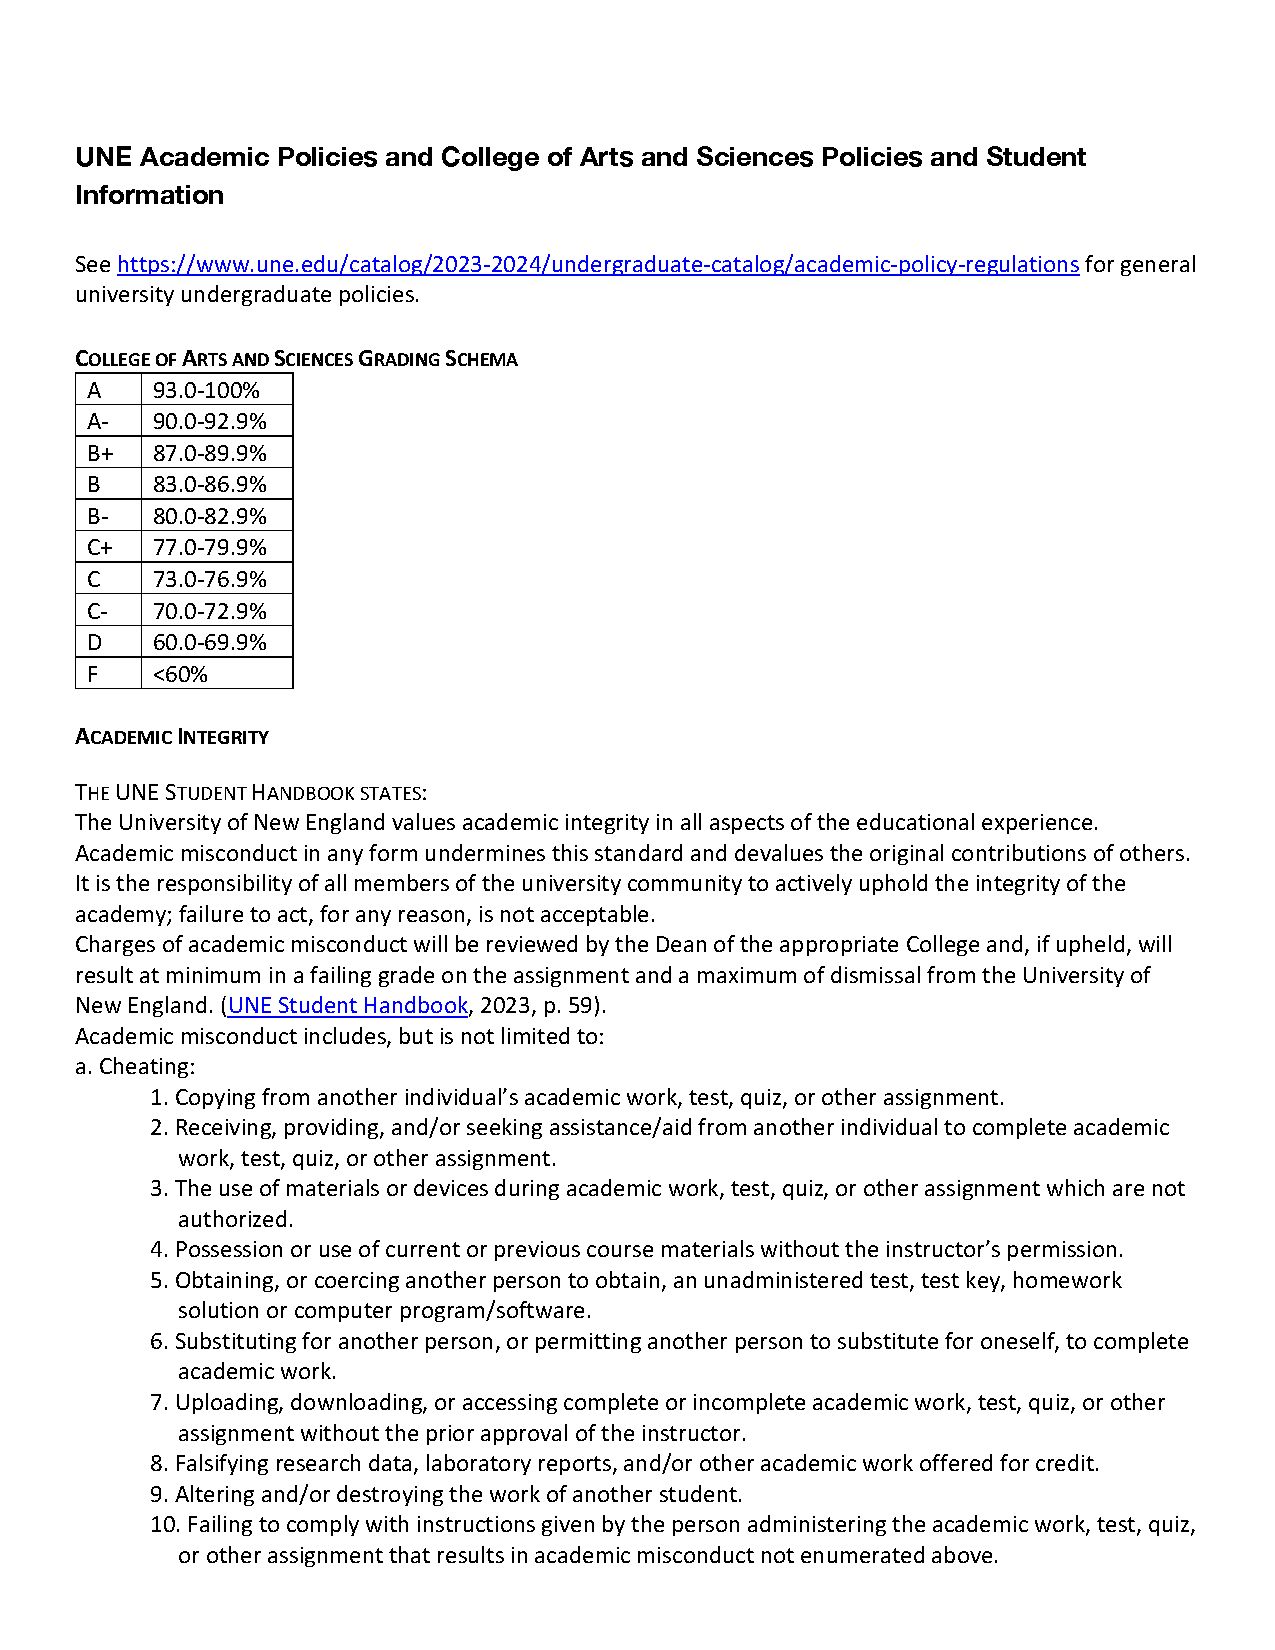
\includepdf[pages={1-3}]{Syllabus_boil.pdf}





\end{document}

